\begin{figure}[ht]
  \centering
  \begin{subfigure}[b]{0.24\textwidth}
    \centering
    
\begin{tikzpicture}
      \draw[thick,red,dashed,fill=red!10] (0,0) circle (1);
    \end{tikzpicture}
    \caption{Simple}
    \label{fig:simple_simple}
  \end{subfigure}
  \hfill
  \begin{subfigure}[b]{0.24\textwidth}
    \centering
    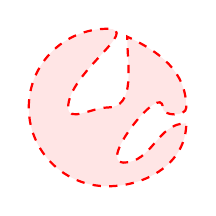
\begin{tikzpicture}
      \draw[thick,red,dashed,fill=red!10] (-1,0) to [out=90,in=180] (0,1)
      to [out=0,in=90] (-0.5,0)
      to [out=270,in=180](0,0)
      to [out=0,in=270] (0.25,0.9)
      to [out=335,in=90] (1,0)
      to [out=270,in=270] (0.7,0)
      to [out=90,in=180] (0.2,-0.7)
      to [out=0,in=180] (1,-0.2)
      to [out=270,in=0] (0,-1)
      to [out=180,in=270] (-1,0);
    \end{tikzpicture}
    \caption{Simple}
    \label{fig:simple_complicada}
  \end{subfigure}
  \hfill
  \begin{subfigure}[b]{0.24\textwidth}
    \centering
    
\begin{tikzpicture}
      \draw[thick,red,dashed,fill=red!10] (0,0) circle (1);
      \draw[thick,red,dashed,rotate=-20,fill=white] (0,0) ellipse [x radius=15pt,y radius=10pt];
    \end{tikzpicture}
    \caption{Doble}
    \label{fig:doblemente_conexo}
  \end{subfigure}
  \hfill 
  \begin{subfigure}[b]{0.24\textwidth}
    \centering
    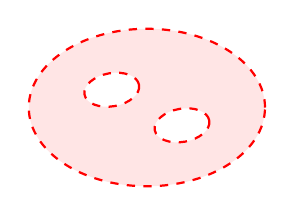
\begin{tikzpicture}
      \draw[thick,red,dashed,fill=red!10] (0,0) ellipse [x radius=1.5, y radius=1];
      \draw[thick,red,dashed,rotate=10,fill=white] (-0.4,0.3) ellipse [x radius=10pt,y radius=6pt];
      \draw[thick,red,dashed,rotate=10,fill=white] (0.4,-0.3) ellipse [x radius=10pt,y radius=6pt];
    \end{tikzpicture}
    \caption{Triple}
    \label{fig:triplemente_conexo}
  \end{subfigure}
  \caption{Conexidad de dominios}
\end{figure}
